% !TeX spellcheck = de_DE

\chapter{GIS Verschneidung}



\section{Mögliche Fragestellungen}
\begin{itemize}
	\item Wie können Vektor und Rasterdaten miteinander verschnitten werden?
	\item Wie können aus der Verschneidung von Datensätzen neue Informationen gewonnen werden?
	\item Wie können Informationen von überlappenden Datensätzen in Mars genutzt werden?
\end{itemize}



\section{Motivation}
Das MARS LIFE Simulationssystem benötigt für die Initialisierung verschiedene Typen von spatialen Daten. Die Eingabedaten müssen den zu simulierenden Bereich abdecken. Derzeit bietet das System keine Möglichkeit Daten auf ihre Kompatibilität hinsichtlich des abgedeckten Bereiches zu prüfen. Dieser Vorgang muss vom Modellentwickler geleistet werden.\\
Ziel dieser Arbeit ist es eine Möglichkeit zur spatialen Einschränkung und Fusion unterschiedlicher Datensätze bereit zu stellen. Hierbei sollen folgende Szenarien abgedeckt werden.


\subsection{Datenreduktion}
Reduktion von Daten auf einen gemeinsamen Bereich.
\begin{enumerate}
	\item Angleichung des Coordinate Reference System (CRS)
	\item Ermittlung der Überschneidungsfläche von Raster- und Vektoreingabedaten.
	\begin{enumerate}
		\item Vektor Polygon der Umrisse von Vektor und Raster Datensatz erstellen
	\end{enumerate}
	\item Reduktion von Datensätzen auf die ermittelte Überschneidungsfläche.
	\begin{enumerate}
		\item Datensatz A und B auf Polygon beschneiden.
	\end{enumerate}
\end{enumerate}

\begin{figure}[H]
	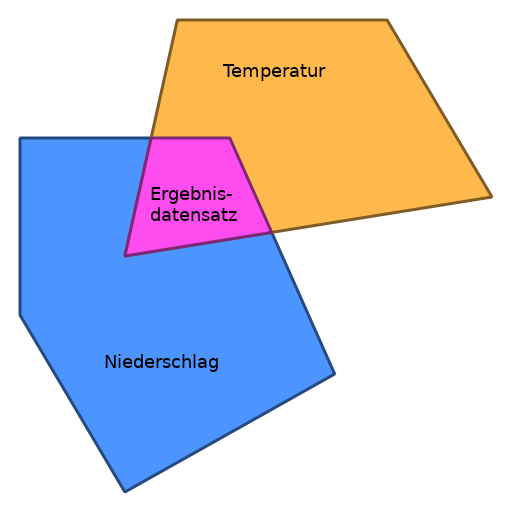
\includegraphics[width=0.5\textwidth]{res/Reduktionsbeispiel}
	\caption{Reduktionsbeispiel}
	\label{fig:Reduktionsbeispiel}
\end{figure}


\subsection{Informationsgewinnung aus Verschneidung (Remote Sensing)}
Informationsgewinnung aus Verschneidung von Datensätzen wie von \cite{Baldowski2014} in Kapitel 5.4 beschrieben (Mögliches Master Thema).\\
Hier ist ein genauer Usecase mit der entsprechenden Fachlichkeit von Nöten.

\begin{figure}[H]
	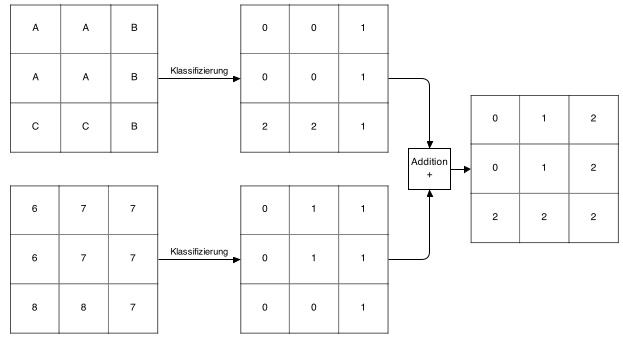
\includegraphics[width=.75\textwidth]{res/Verschneidung}
	\caption{Verschneidung nach Baldowski}
	\label{fig:Verschneidung}
\end{figure}


\section{Paper}
\begin{itemize}
	\item \textbf{A spatial data partitioning and merging method for parallel vector spatial analysis}: \cite{Qiu2015}
	\item \textbf{Räumliche Analyse mit spatialen Indikatoren}: \cite{Baldowski2014}
	\item \textbf{MapSnap system to perform vector-to-raster fusion}: \cite{Kovalerchuk2011}
	\item \textbf{Multi-source remote sensing data fusion: status and trends}: \cite{Zhang2010}
	\item \textbf{Mathematical support for combining geospatial data}: \cite{Kovalerchuk2001}
\end{itemize}
